%
% QTCP Protocol Stack
%

\subsection{QTCP protocol stack} \label{sec:prot_stack} \index{QTCP protocol stack}

As with classical networking, our protocols for quantum networks will be separated into distinct layers, each performing a specific set of tasks with different levels of abstraction.

The structure of the protocol stack for QTCP is shown in Fig.~\ref{fig:stack}. In summary, the layers in the protocol stack are, beginning from the lowest level:
\begin{itemize}
\item \textsc{Data (Message)}\index{Data (message) layer}: Raw data (`payload') Alice wishes to transmit to Bob. Comprises both \textsc{Quantum Data}\index{Quantum data layer} and \textsc{Classical Data}\index{Classical data layer}.
\item \textsc{Packet}\index{Packet!Layer}: Decomposition of \textsc{Data} into blocks (\textsc{Packet Data}\index{Packet!Data layer}), and associated classical \textsc{Packet Headers}\index{Packet!Header layer} containing metadata (e.g routing information).
\item \textsc{Strategy}\index{Strategy!Layer}: Construct \textsc{Packet} routing strategies based on a cost optimisation algorithm.
\item \textsc{Transport}\index{Transport layer}: Physical routing of \textsc{Packets} to arrive at their destination, based upon metadata contained in \textsc{Packet Header}. Perform collision detection during transit.
\item \textsc{Reconstruction}\index{Reconstruction layer}: Reconstruct \textsc{Data} from received \textsc{Packets}.
\item \textsc{Quality of Service (QoS)}\index{Quality of service (QoS) layer}: Apply QEC and determine whether \textsc{QoS} requirements have been satisfied.
\item \textsc{Services \& Applications}\index{Services \& applications layer}: High-level interface to \textsc{Data} presented to Bob's services and applications. The interface abstracts away lower levels of the protocol stack, presenting Bob with only \textsc{Data} and its associated metadata.
\end{itemize}

\begin{figure}[!htbp]\index{QTCP protocol stack}
\if 2\pubmode
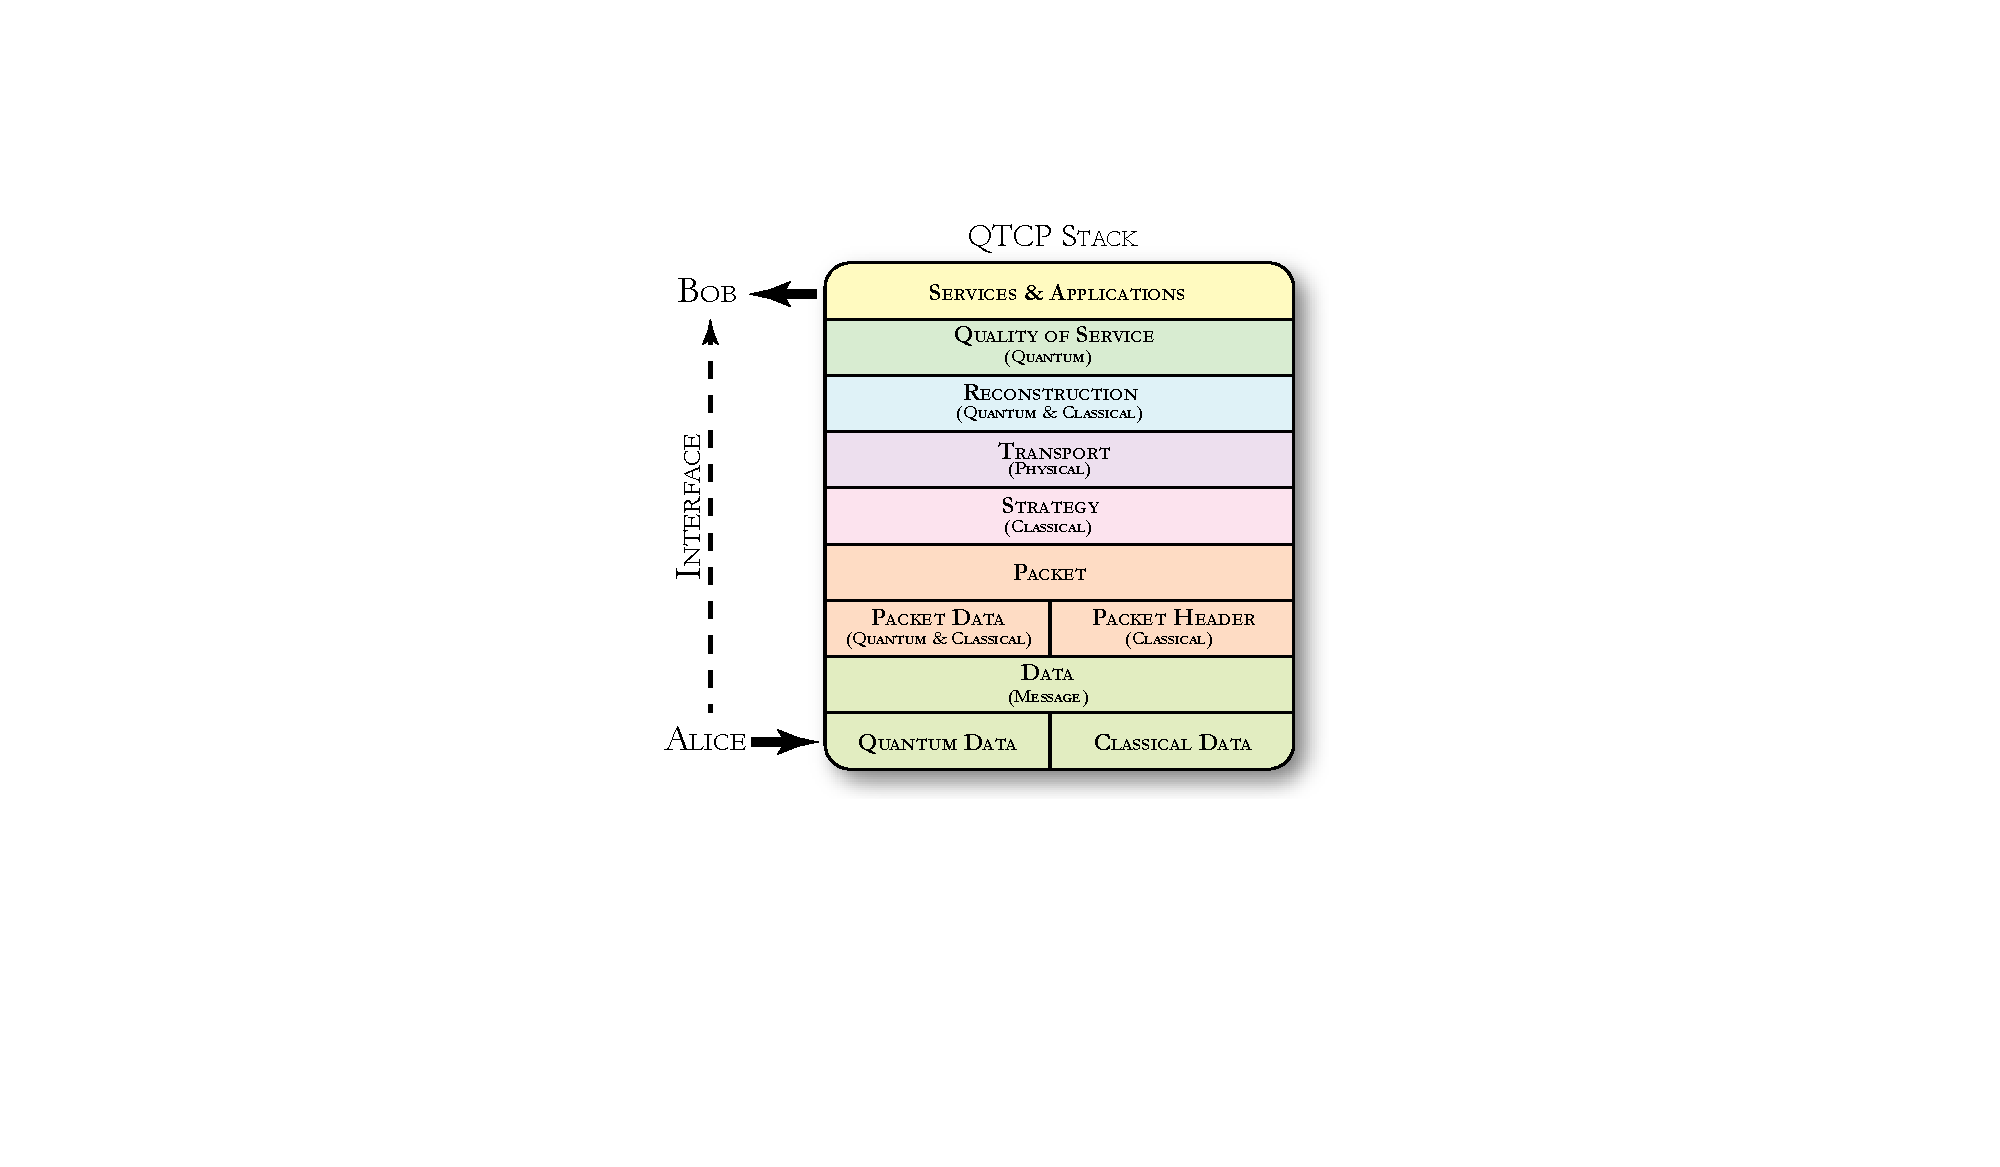
\includegraphics[clip=true, width=0.475\textwidth]{stack}
\else
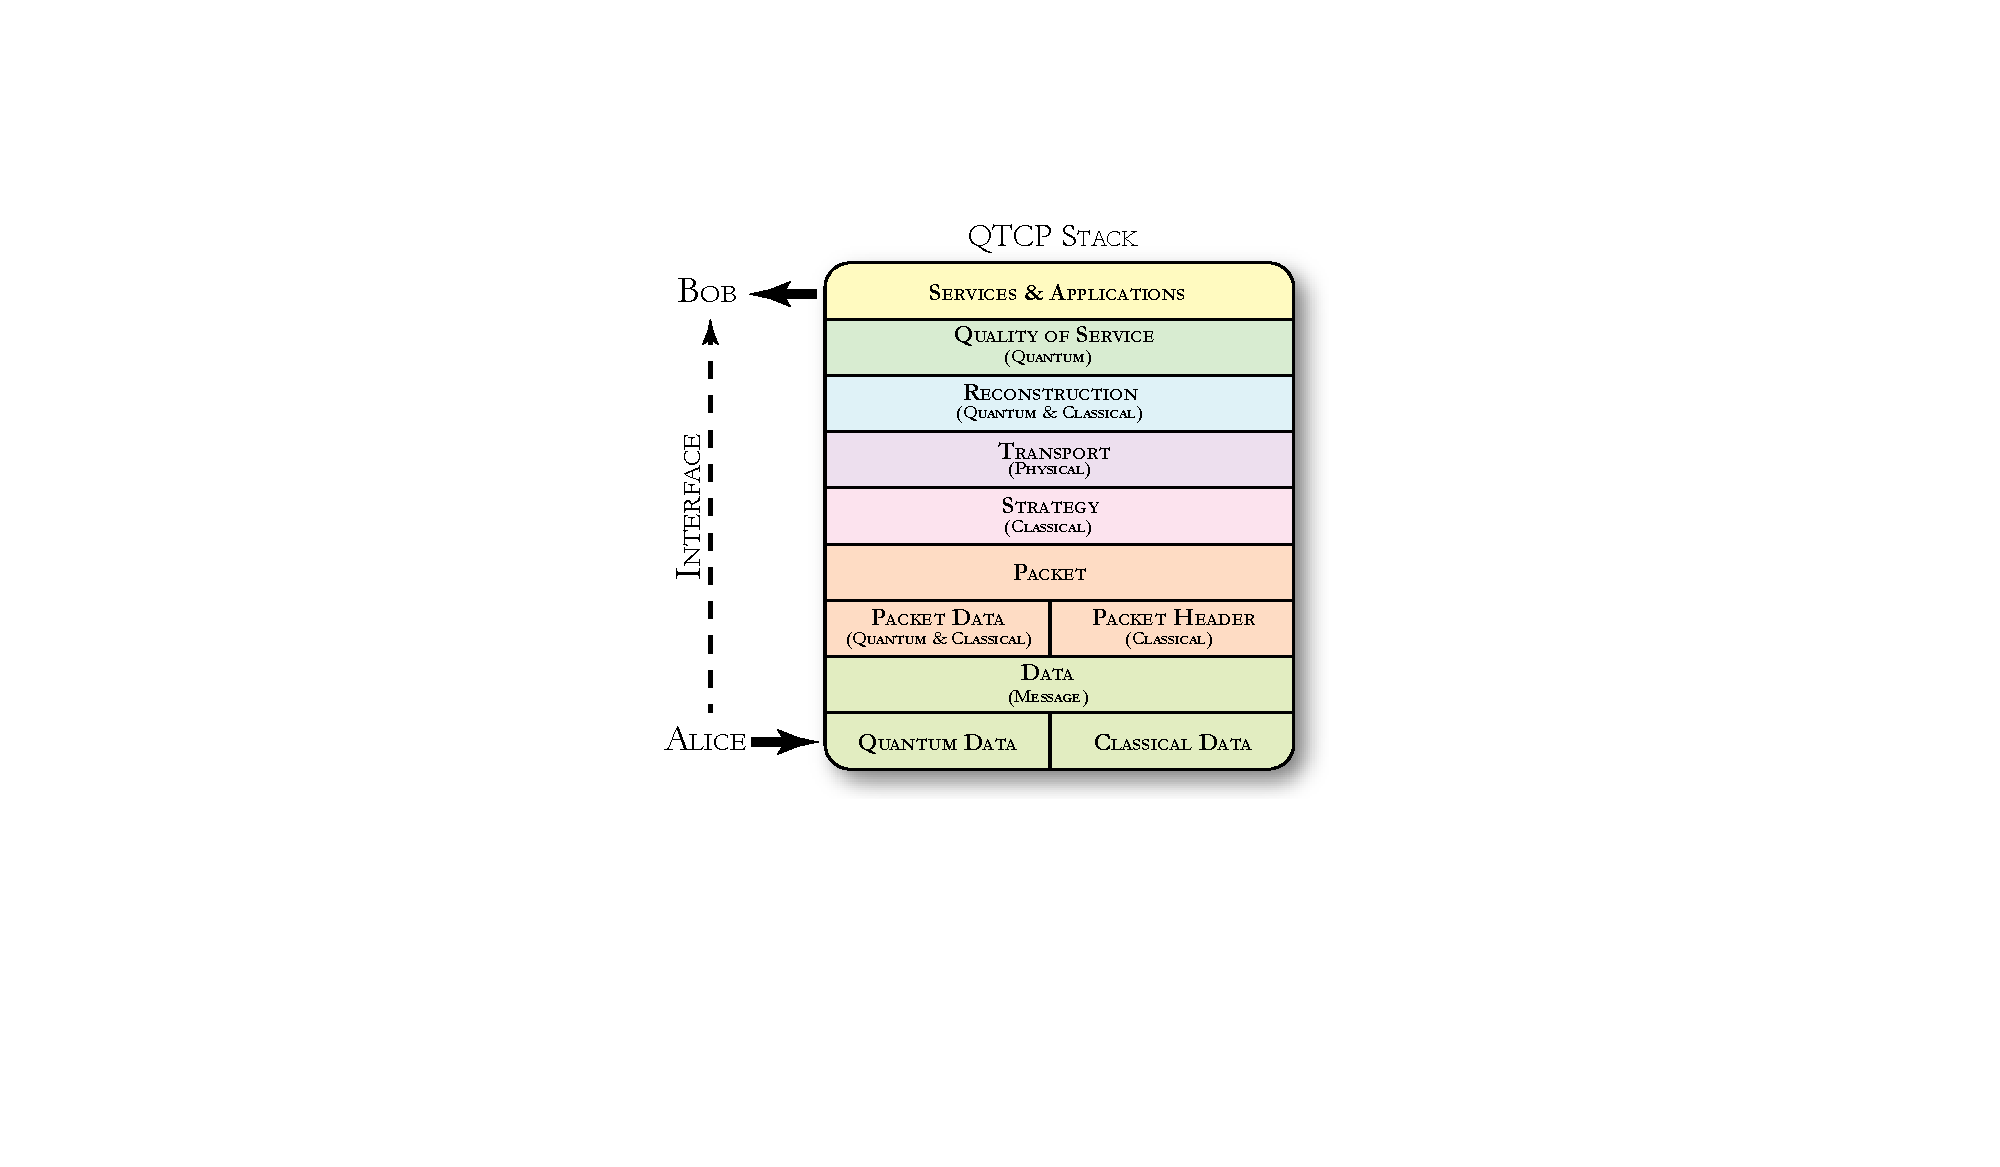
\includegraphics[clip=true, width=0.6\textwidth]{stack}
\fi
\captionspacefig \caption{Protocol stack for QTCP. The protocol stack mediates communication of quantum data from Alice to Bob using the shown layers of abstraction. The end goal is to provide Bob a virtual interface to Alice's transmitted data, while remaining oblivious to the underlying protocol.} \label{fig:stack}\index{QTCP protocol stack}
\end{figure}

Next we describe the operation of these layers in detail.

%
% Data (Message)
%

\subsubsection{Data (Message)} \index{Data (message) layer} \label{sec:data_message_layer}

At the lowest level of the protocol we have the raw \textsc{Data} Alice wishes to communicate to Bob. \textsc{Data} is allowed to comprise both \textsc{Quantum Data} and \textsc{Classical Data} components, and may contain one or the other, or both.

%
% Quantum Data
%

\paragraph{Quantum data} \index{Quantum data layer}

\textsc{Quantum Data} is allowed to be an arbitrary quantum state. It could be a pure or mixed state, of arbitrary (but predetermined) dimension, or even a subsystem of a larger external state (i.e entangled with another system). We stress that it needn't be expressed using a conventional qubit representation, in the way digital data is necessarily represented using bits. Keep in mind that the quantum internet isn't just there to communicate qubit data streams. Rather, it is intended to act as generally as possible, such that essentially arbitrary \textit{quantum assets}\index{Quantum assets} can be exchanged. These needn't be restricted to any particular type of encoding, such as those discussed in Sec.~\ref{sec:opt_enc_of_qi}. For example, in addition to something `standard' like polarisation-encoded qubits in single photons, one network user might like to share an exotic CV state of light, like a cat state, with his mate whose cat died. Indeed, multiple types of state encoding might be encapsulated within a single \textsc{Packet}. The QTCP acts only as an abstract interface for quantum networking, but is completely blind as to what the underlying data in the network is. QTCP is only concerned with getting that state from Alice to Bob.

%
% Classical Data
%

\paragraph{Classical data} \index{Classical data layer}

\textsc{Classical Data} is a purely classical state with no coherence (i.e a diagonal density matrix), which may be represented as a classical bit-string. We very intentionally segregate the \textsc{Classical} and \textsc{Quantum} components of \textsc{Data}, since the classical network is expected to be cheaper and more reliable than the quantum network operating in parallel to it. The \textsc{Classical Data} could, for example, provide nodes with classical instructions on what quantum computations to perform on the \textsc{Quantum Data}.

%
% Packet
%

\subsubsection{Packet} \label{sec:packet_layer} \index{Packet!Layer}

\textsc{Data} is transmitted as \textsc{Packets}, much in the same way as conventional TCP. The \textsc{Data} is decomposed into three components: \textsc{Quantum Data}, \textsc{Classical Data}, and \textsc{Packet Header}.

We can express the state of an entire \textsc{Packet} as,
\begin{align}
\hat\rho_\mathrm{packet}(i) = \hat\rho_\mathrm{quantum}(i) \oplus \hat\rho_\mathrm{classical}(i) \oplus \hat\rho_\mathrm{header}(i),
\end{align}
where $i$ denotes the $i$th packet. Here $\hat\rho_\mathrm{quantum}$ ($\hat\rho_\mathrm{classical}$) is a block of \textsc{Quantum Block Size} qubits (\textsc{Classical Block Size} bits) taken from the user's \textsc{Quantum Data} (\textsc{Classical Data}), while $\hat\rho_\mathrm{header}$ is the \textsc{Packet's} classical \textsc{Packet Header}. As discussed earlier, since $\hat\rho_\mathrm{quantum}$ is quantum, and $\hat\rho_\mathrm{classical}$ and $\hat\rho_\mathrm{header}$ are classical, they needn't be transmitted together over the same quantum network. Instead all \textsc{Classical Data} and \textsc{Packet Header} could be transmitted over a classical network operating in parallel to and synchronised with the quantum network, which carries the \textsc{Quantum Data}.

Note that while one can always measure classical data without disturbance, this is not the case with quantum data, where measurements cause wavefunction collapse. Thus, while Alice is always able to know $\hat\rho_\mathrm{classical}$ and $\hat\rho_\mathrm{header}$, she may or may not know $\hat\rho_\mathrm{quantum}$. Clearly if she prepared the state herself, she would (hopefully) know what she was doing. But in general, quantum networks could be used for far less trivial networking, where Alice is, for example, an intermediary in a distributed quantum computation. In this instance, Alice is unlikely to know what her \textsc{Quantum Data} is.

%
% Packet Data
%

\paragraph{Packet data} \index{Packet!Data layer}

Comprises blocks of both \textsc{Quantum Data} and \textsc{Classical Data}, of sizes \textsc{Quantum Block Size} and \textsc{Classical Block Size} respectively. \textsc{Packet Data} requires that \textsc{Data} be decomposed into distinct subsystems which are independently transmitted by QTCP. For easy of exposition, we will restrict ourselves to the case where the \textsc{Data} is encoded into a stream of qubits (\textsc{Quantum Data}) and bits (\textsc{Classical Data}). But of course other encodings could be used. Also bear in mind that any quantum (classical) information can be encoded into qubits (bits), and once represented as such, the decomposition of \textsc{Data} into \textsc{Packets} arises very naturally and intuitively. The \textsc{Packet's} \textsc{Quantum Data} is what is transmitted via the quantum channels, while the \textsc{Classical Data} is communicated via classical channels.

%
% Packet Header
%

\paragraph{Packet header} \label{sec:packet_header} \index{Packet!Header layer}

\textsc{Packet Header} is purely classical and needn't be transmitted over the costly quantum network, instead being transmitted over a complementary classical network, running in parallel to, and synchronised with the quantum network. \textsc{Packet Header} contains no information content from \textsc{Data}, instead comprising only metadata relevant to the higher levels of the protocol stack. In particular, \textsc{Packet Header} contains the following fields:
\begin{itemize}
    \item \textsc{Header Size}\index{Header size}: The number of bits in the \textsc{Packet Header}.
    \item \textsc{Message ID}\index{Message ID}: A unique identifier for the complete message to which this \textsc{Packet} belongs. This field mitigates ambiguity as to which \textsc{Message} this packet belongs when performing \textsc{Reconstruction}.
    \item \textsc{Lifetime}\index{Lifetime}: How long the \textsc{Packet} has been in existence for, i.e since it was initially sent by the \textsc{Sender}. This is used by strategies to prevent collisions.
    \item \textsc{Sender}\index{Sender}: A unique node identifier for the sender (Alice).
    \item \textsc{Recipient}\index{Recipient}: A unique node identifier for the recipient (Bob).
    \item \textsc{Order}\index{Order}: To which block taken from \textsc{Data} does this \textsc{Packet Data} belong? This is extremely important in networks where \textsc{Packets} may arrive out of order. The \textsc{Order} field forms the basis for the \textsc{Reconstruction} layer.
    \item \textsc{Quantum Block Size}\index{Quantum block size}: The number of qubits contained in the \textsc{Quantum} component of \textsc{Packet Data}. This is important for the \textsc{Reconstruction} layer.
    \item \textsc{Classical Block Size}\index{Classical block size}: The number of bits contained in the \textsc{Classical} component of \textsc{Packet Data}, also important for the \textsc{Reconstruction} layer.
    \item \textsc{Routing Queue}\index{Routing!Queues}: A first in, first out (FIFO) queue of node identifiers, tracing out the entire route for the \textsc{Packet} to follow, in chronological order from the next node to visit all the way to the \textsc{Recipient}.
    \item \textsc{Costs}\index{Costs}: A tuple characterising all the accumulated costs of the \textsc{Packet} at the current stage in the route. These are treated as accumulators that are incremented appropriately after each step, since costs are additive.
    \item \textsc{Attributes}\index{Attributes}: A tuple characterising all the non-\textsc{Cost} properties associated with the \textsc{Packet}. Examples include: the \textsc{Priority} of routing a \textsc{Packet} to its destination; suggesting a preferred routing \textsc{Strategy}; or, indicating whether or not a \textsc{Resend Until Success} protocol may be applied to this \textsc{Packet}.
    \item \textsc{Padding}\index{Padding}: Null data to pad the joint \textsc{Classical Packet Data} and \textsc{Packet Header} fields to be of the same length as the \textsc{Quantum Packet Data}. This ensures that the components of the \textsc{Packet} traversing the quantum and classical channels remain in perfect tandem -- bit for qubit. In Sec.~\ref{sec:transport} we show that this facilitates collision detection without the need to measure quantum states.
    \item \textsc{Checksum}\index{Checksums}: A regular checksum of the entire \textsc{Classical} component of the \textsc{Packet}, including both \textsc{Classical Packet Data} and \textsc{Packet Header}. This also forms a part of the collision detection protocol.
\end{itemize}

One might question why \textsc{Packet Headers} tally accumulated costs when we ought to already know all the costs, since these were employed by the algorithm for choosing strategies in the first case. In the ideal case where all strategies are determined \textit{a priori} and are implemented as intended, this is certainly valid. However, for generality we retain this option since more realistic networks may require dynamically updating strategies during the course of propagation, in which case dynamically tallying costs is appropriate.

%
% Strategy
%

\subsubsection{Strategy} \label{sec:intro_strat} \index{Strategy!Layer}

Based on the \textsc{Packet Headers} of all users sharing the network, choose routing strategies to optimise cost metrics. The notion of strategies is introduced in Sec.~\ref{sec:strat_opt}, and a detailed discussion of example strategies is presented in Sec.~\ref{sec:strategies}.

Once routings have been determined for all \textsc{Packets}, the \textsc{Routing Queues} in their \textsc{Packet Headers} are initialised accordingly by pushing the sequence of node identifiers tracing out the desired route.

In the case of dynamic, time-dependent strategies, which can be updated within the duration of transmissions, the \textsc{Routing Queues} may need to be updated. A change in a \textsc{Packet's} route simply requires flushing the queue and pushing new node identifiers for each of the nodes in the new route, in chronological order.

The \textsc{Strategy} layer is responsible for evaluating the net cost function $f_\mathrm{cost}$ from Eq.~(\ref{eq:net_cost_R}), which accounts for both \textsc{Costs} and \textsc{Attributes} to calculate a single effective cost measure that may be employed in routing decisions.

%
% Transport
%

\subsubsection{Transport} \label{sec:transport} \index{Transport layer}

The \textsc{Transport} layer is responsible for actual routing at the physical level, making direct decisions as to what to do with a \textsc{Packet} at each step, based upon the metadata contained in \textsc{Packet Header}, most notably the \textsc{Routing Queue}, which specifies the full route a \textsc{Packet} is destined to follow. It is also responsible for keeping track of costs that accumulate over their route.

Additionally, the \textsc{Transport} layer is responsible for collision detection, whereby multiple packets being transmitted simultaneously over a network interfere with one another, corrupting the data. In classical networking, collision detection is straightforward using checksums. But the usual classical approach breaks down in the quantum setting. In Sec.~\ref{sec:collision} we discuss in detail collision detection in QTCP.

The pseudo-code algorithm implemented by the \textsc{Transport} layer, including collision detection, is shown in Alg.~\ref{alg:transport_alg}.

\startalgtable
\begin{table}[!htbp]
\begin{mdframed}[innertopmargin=3pt, innerbottommargin=3pt, nobreak]
\texttt{
function Transport(Packet):
\begin{enumerate}
    \item nextNode = Packet.RoutingQueue.Pop()
    \item Packet.PhysicallySendTo(nextNode)
    \item Packet.WaitUntilArrivesAt(nextNode)
    \item checksum = Hash(Packet.Header + Packet.ClassicalData)
    \item if(checksum $\neq$ Packet.Header.Checksum) \{
    \setlength{\itemindent}{0.2in}
    \item Packet.Sender.Notify(\textsc{Failure})
    \item Packet.Recipient.Notify(\textsc{Failure})
    \item Packet.Discard()
    \item $\Box$
        \setlength{\itemindent}{0in}
\item \}
    \item Packet.Costs += IncomingLink.Costs
    \item Packet.Attributes.Update()
    \item if(Packet.RoutingQueue.Length = 0) \{
    \setlength{\itemindent}{0.2in}
    \item Return(Packet)
        \setlength{\itemindent}{0in}
    \item \}
    \setlength{\itemindent}{0in}
    \item $\Box$
\end{enumerate}}
\end{mdframed}
\captionspacealg \caption{Algorithm implemented by the \textsc{Transport} layer of QTCP for each \textsc{Packet}. The \texttt{Attributes.Update()} function is left undefined. This is where arbitrary \textsc{Attribute} dynamics may take place.} \label{alg:transport_alg}
\end{table}

%
% Reconstruction
%

\subsubsection{Reconstruction} \index{Reconstruction layer} \label{sec:reconstruction_layer}

The \textsc{Reconstruction} layer only serves one purpose -- to chronologically reorder the received \textsc{Packets} based on the \textsc{Order} field in their \textsc{Packet Headers}. This stage is only performed by Bob -- the final recipient -- and not at any intermediate stage. In general this will require Bob to have a quantum memory, able to hold all \textsc{Packet Data} for a sufficient duration as to enable an arbitrary permutation of \textsc{Packets} to be applied, reproducing the correct chronological order. The algorithm for this is shown in Alg.~\ref{alg:reconstruction}.

\begin{table}[!htbp]
\begin{mdframed}[innertopmargin=3pt, innerbottommargin=3pt, nobreak]
\texttt{
function Reconstruction(Packets):
\begin{enumerate}
    \item Packets.WaitUntilAllReceived()
    \item message =\\ 
    Packets.SortByOrderAscending().data
    \item Packets.Receiver.Notify(message)
     \item $\Box$
\end{enumerate}}
\end{mdframed}
\captionspacealg \caption{The goal of the \textsc{Reconstruction} layer, is to take a collection of received \textsc{Packets} and reassemble them into the \textsc{Message}.} \label{alg:reconstruction}
\end{table}

%
% Quality of Service (QoS)
%

\subsubsection{Quality of service} \label{sec:QOS} \index{Quality of service (QoS) layer}

In classical networking theory, error detection and correction is an important element of networking protocols. Communication links may be unreliable, or subject to external noise, which users must be able to detect so as to guarantee the quality of their data.

Classically, error detection is typically performed using checksums (hash functions), which generate a short digest of a packet's data that can be recalculated upon arrival to verify integrity. The checksum can be included in the header component of each packet, allowing the remainder of the protocol to remain unchanged.

In the quantum context the elegant notion of checksums is complicated by the fact that calculating a hash function of a quantum state would necessarily entangle the state with the output hash. This would have the undesired effect of causing measurement of the checksum to collapse the quantum state of the data, thereby altering it in an uncontrollable way.

As an alternative to checksums, we could borrow the notion of quantum error correction (QEC)\index{Quantum error correction (QEC)} and fault-tolerance\index{Fault-tolerance} from quantum computing theory \cite{???}. Here we encode a quantum state into a (polynomially) larger Hilbert space. \textit{Syndrome measurements}\index{Syndromes!Measurements} on some of the states in this larger space allow us to both detect and correct universal error models, such as depolarisation or dephasing, provided that error rates are within the fault-tolerance threshold of the code being employed.

Thus, enforcing QoS in fundamentally different for quantum data packets than for classical ones, requiring entirely different techniques. Given how large a field this has become in its own right, we dedicate Sec.~\ref{sec:QOS_chap} entirely to protocols suited to the implementation of quantum QoS requirements in quantum networks.

%
% Services & Applications
%

\subsubsection{Services \& applications} \index{Services \& applications layer} \label{sec:services_apps}

Having communicated all the \textsc{Packet Data} from Alice to Bob, performed \textsc{Reconstruction}, and applied \textsc{QoS} protocols, Bob ought to have $\hat\rho_\mathrm{data}$ to a good approximation. The quality of Bob's received state can be inferred directly from the \textsc{Costs} vector contained in the \textsc{Packet Headers}. The final state and its associated quality metrics (\textsc{Costs} and QEC outcomes) may then be provided to Bob as a software interface for end use.